\chapter{Evolução Molecular e Filogenômica}\label{ch:b3:molecular-evolution}

Em 1968 Motoo Kimura fez uma conta que abalou um campo. Comparando as
hemoglobinas, os citocromos e outras proteínas de mamíferos cujos
ancestrais comuns estavam datados por fósseis, ele descobriu que os
aminoácidos tinham sido substituídos a uma taxa de cerca de uma
substituição por sítio por bilhão de anos --- o que, num genoma de
mamífero e numa geração, dava uma nova substituição fixada na população a
cada dois anos mais ou menos. Haldane havia mostrado, uma década antes,
que a seleção natural consegue fixar no máximo cerca de uma substituição
a cada trezentas gerações antes que o custo em prole perdida se torne
impagável. A aritmética deixava uma só saída: a maior parte das mudanças
que se acumulam no DNA não é movida por seleção alguma, mas é neutra,
fixada por acaso em populações finitas, a uma taxa que --- como mostra o
primeiro teorema deste capítulo --- é simplesmente a taxa de mutação. A
\omterm{thm:b3:molecular-evolution:neutral}{teoria neutra} virou a hipótese nula da evolução molecular, a linha de
base contra a qual a seleção é detectada; o \omterm{prop:b3:molecular-evolution:clock}{relógio molecular} virou um
modo de datar o que os fósseis não datavam; e os genomas sequenciados
desde então deram as ferramentas para ver, gene a gene, onde a seleção
agiu, como genes novos nascem de velhos e por que a árvore de um gene
nem sempre é a árvore de sua espécie.

\section{Deriva, mutação e a taxa neutra}

\begin{theorem}[A taxa neutra de substituição]\label{thm:b3:molecular-evolution:neutral}
\index{teoria neutra}\index{taxa de substituição}\index{probabilidade de fixação}\index{deriva genética}
Numa população diploide de $N$ indivíduos, uma mutação nova sem efeito
sobre a aptidão tem probabilidade $1/2N$ de acabar substituindo todos os
outros alelos (\emph{fixação}) e $1 - 1/2N$ de ser perdida. Se cada uma
das $2N$ cópias gênicas muta à taxa $\mu$ por geração, surgem $2N\mu$
mutações neutras novas por geração e, no longo prazo, a taxa em que as
substituições se acumulam é
\[
k = 2N\mu\times\frac{1}{2N} = \mu :
\]
a \emph{\omterm{thm:b3:molecular-evolution:neutral}{taxa de substituição}} neutra é igual à taxa de mutação,
independentemente do tamanho da população. Uma mutação destinada a se
fixar leva em média $4N$ gerações para tanto, de modo que populações
grandes guardam mais variação em trânsito, mas não a fixam mais depressa.
Para uma mutação com vantagem seletiva $s$, a fórmula de Kimura dá a
\omterm{thm:b3:molecular-evolution:neutral}{probabilidade de fixação}
\[
P(s) = \frac{1 - \mathrm{e}^{-2s}}{1 - \mathrm{e}^{-4Ns}} \approx 2s
\quad (4Ns \gg 1),
\]
de modo que uma vantagem de \qty{1}{\%} se fixa com probabilidade de
cerca de \qty{2}{\%} --- quarenta vezes a chance de uma mutação neutra
numa população de dois mil, mas ainda assim perdida quarenta e nove vezes
em cinquenta; e uma desvantagem $s < 0$ com $4N|s| \gg 1$ praticamente
nunca se fixa, enquanto uma com $4N|s| \ll 1$ se comporta como neutra: a
seleção só vê o que a deriva não engole, e a fronteira é $|s| \sim
1/4N$
--- \emph{efetivamente neutra}.
\end{theorem}
\begin{proof}
Neutralidade: alguma cópia presente hoje será a ancestral de toda a
população num futuro distante e, por simetria, cada uma das $2N$ cópias
tem igual chance de ser ela; a mutante nova é uma cópia, daí $1/2N$.
Taxa: substituições por geração $=$ (mutações surgidas por geração)
$\times$ (probabilidade de cada uma se fixar) $= 2N\mu/2N$. A fórmula de
Kimura decorre da aproximação por difusão da variação da frequência
alélica sob deriva e seleção, aqui admitida; seus limites se verificam
diretamente: quando $s \to 0$, $(2s)/(4Ns) = 1/2N$, o valor neutro; para
$4Ns \gg 1$ o denominador é $1$ e o numerador, $\approx 2s$. Tempo de
fixação: a frequência de um alelo neutro faz um passeio aleatório com
variância $p(1-p)/2N$ por geração, e o tempo esperado para chegar a $1$
a partir de $1/2N$, condicionado a isso acontecer, é de $4N$ gerações
(Kimura e Ohta, 1969), admitido.
\end{proof}

\begin{omfigure}
\begin{tikzpicture}
\begin{semilogyaxis}[
  width=0.62\linewidth, height=5.6cm,
  axis x line=bottom, axis y line=left,
  xmin=-4, xmax=8, ymin=0.00002, ymax=0.2,
  xlabel={$4Ns$ (coeficiente de seleção escalonado)}, ylabel={probabilidade de fixação},
  xlabel style={font=\small, at={(axis description cs:0.5,-0.12)}, anchor=north}, ylabel style={font=\small},
  tick label style={font=\small}, xtick={-4,-2,0,2,4,6,8}, ytick={0.0001,0.001,0.01,0.1}, yticklabels={$10^{-4}$,$10^{-3}$,$10^{-2}$,$10^{-1}$},
  clip=false,
]
\addplot[very thick, omDef, domain=-4:-0.05, samples=60] {(x/2000)/(1-exp(-x))};
\addplot[very thick, omDef, domain=0.05:8, samples=80] {(x/2000)/(1-exp(-x))};
\draw[dashed, gray] (axis cs:-4,0.0005) -- (axis cs:8,0.0005); \node[font=\scriptsize, gray, anchor=north west] at (axis cs:-3.9,0.00048) {neutra, $1/2N$};
\addplot[thick, omThm, dashed, domain=1:8, samples=2] {2*x/(4*1000)};
\node[font=\scriptsize, omThm, anchor=north west] at (axis cs:5,0.0012) {assíntota $2s$};
\node[font=\scriptsize, omDef, anchor=south east, align=right] at (axis cs:-0.2,0.02) {efetivamente neutra\\quando $|4Ns| \lesssim 1$};
\node[font=\scriptsize, omDef, anchor=south west] at (axis cs:-3.9,0.0008) {deletéria: quase nunca se fixa};
\end{semilogyaxis}
\end{tikzpicture}

{\small A \omterm{thm:b3:molecular-evolution:neutral}{probabilidade de fixação} de Kimura em função do coeficiente de
seleção escalonado, para $N = 1000$. Perto de zero a curva passa pelo
valor neutro; à direita ela sobe rumo a $2s$; à esquerda ela despenca. A
seleção só age sobre o que a deriva não consegue esconder.}
\end{omfigure}

\begin{proof}[Evidência]
Kimura (1968) e King e Jukes (1969) fizeram o argumento a partir das
taxas: a taxa observada de substituição de aminoácidos nas proteínas dos
mamíferos implicava mais substituições por geração do que o custo da
seleção de Haldane permitia, de modo que a maioria tinha de ser neutra. As
previsões da teoria então se confirmaram: as taxas são mais altas onde a
função é menos restrita --- sítios sinônimos, íntrons, \omterm{def:b3:molecular-evolution:duplication}{pseudogenes}, a
terceira posição do códon --- e mais baixas nas \omterm{def:b3:chromatin-epigenetics:nucleosome}{histonas} e na ubiquitina,
que mudam um resíduo a cada cem milhões de anos; o nível de variação
dentro das espécies acompanha a mutação e o tamanho populacional; e a
\omterm{thm:b3:molecular-evolution:neutral}{taxa de substituição} por ano é aproximadamente constante entre linhagens
com tamanhos populacionais muito diferentes, como a fórmula $k = \mu$
exige e uma explicação selecionista não. A controvérsia que se seguiu não
a derrubou: ela fixou a taxa neutra como a hipótese nula contra a qual se
mede a seleção.
\end{proof}

\begin{omfigure}
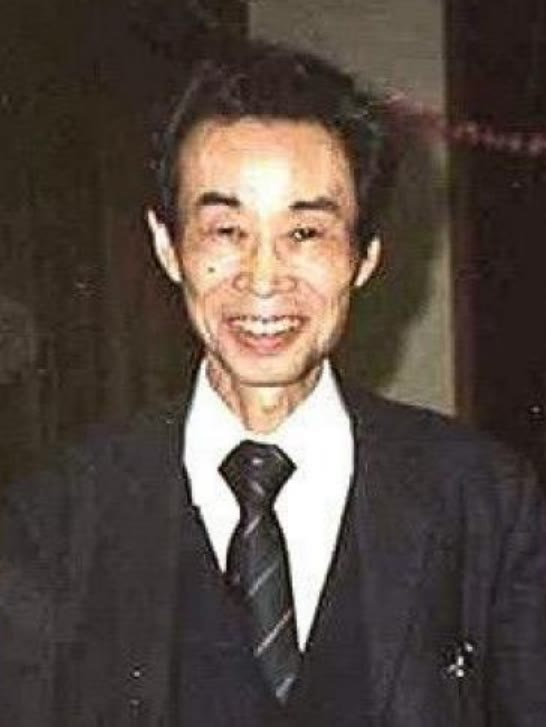
\includegraphics[width=0.34\linewidth]{images/book5/kimura.jpg}\hspace{0.05\linewidth}
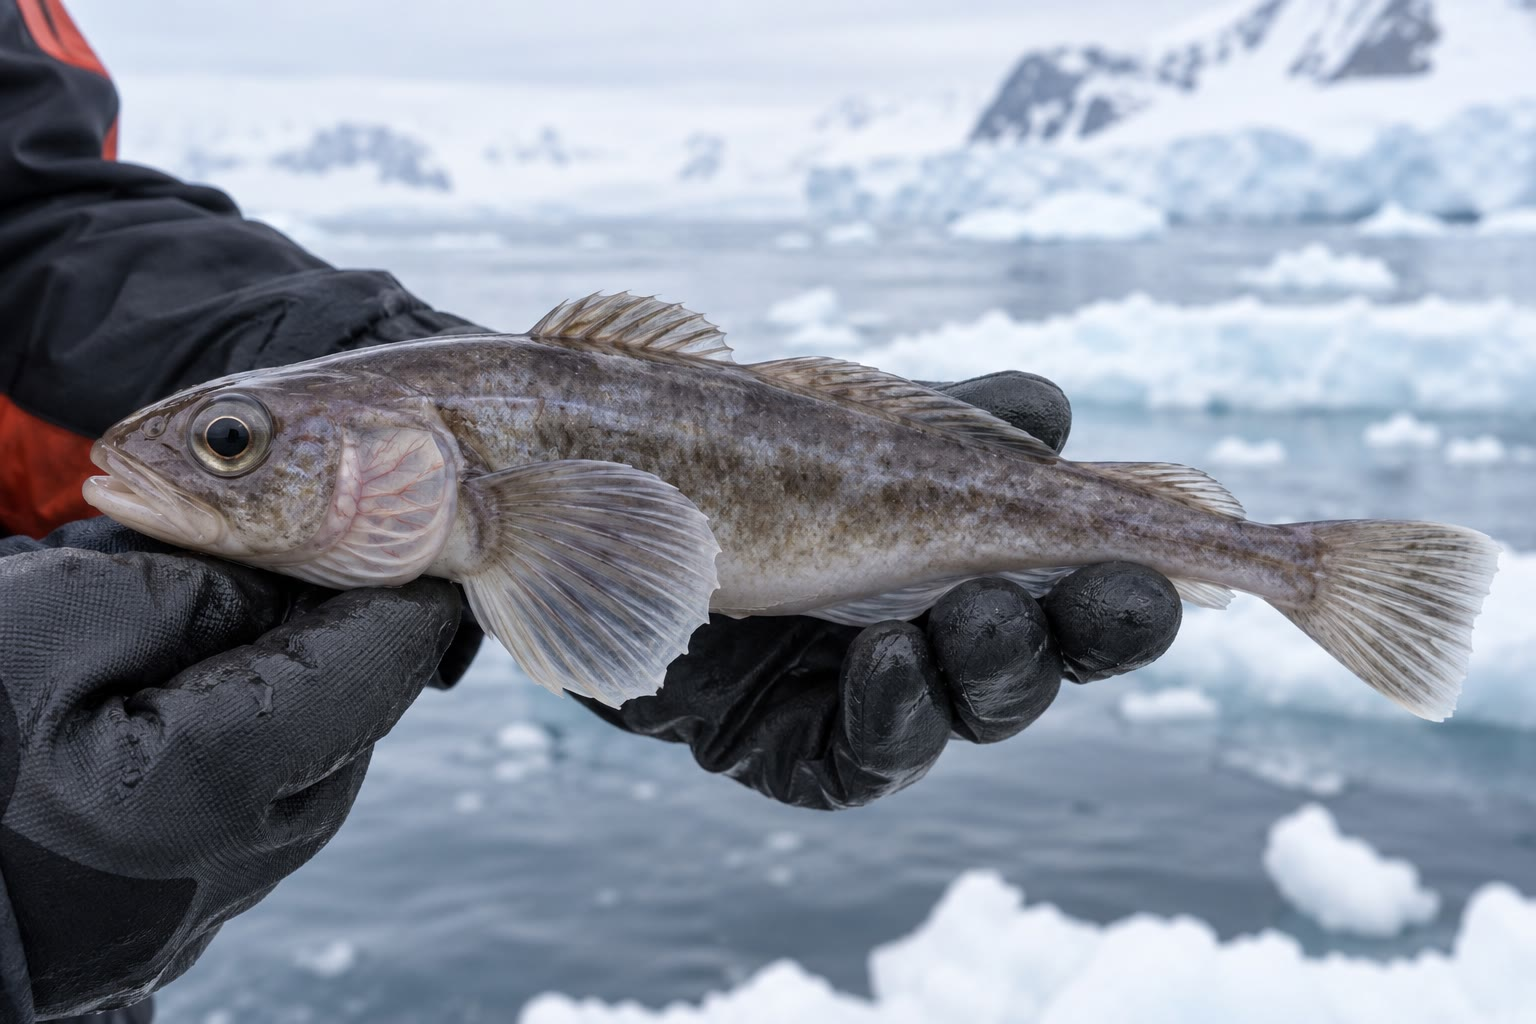
\includegraphics[width=0.5\linewidth]{images/book5/ai/b5-25-icefish.jpg}

{\small À esquerda: Motoo Kimura (1924--1994), que mostrou que a maior
parte da mudança molecular é fixada por acaso e na taxa de mutação
(fotografia, 1986, CC BY 4.0). À direita: um peixe-gelo antártico, cujo
sangue é impedido de congelar por uma glicoproteína anticongelante
montada, uns dez milhões de anos atrás, a partir de um gene duplicado de
enzima digestiva e de uma sequência de repetições.}
\end{omfigure}

\section{O relógio molecular}

\begin{proposition}[O relógio e suas irregularidades]\label{prop:b3:molecular-evolution:clock}
\index{relógio molecular}\index{calibração}\index{heterogeneidade de taxas}\index{relógio relaxado}\index{efeito do tempo de geração}
Se as substituições se acumulam a uma taxa constante $k$ por sítio por
ano em duas linhagens que se separaram há $T$ anos, a fração de sítios em
que elas diferem é, para valores pequenos, $d \approx 2kT$: a divergência
de duas sequências é um \emph{\omterm{prop:b3:molecular-evolution:clock}{relógio molecular}} (Zuckerkandl e Pauling,
1965), que pode ser \emph{calibrado} por uma separação datada por fóssil
e então lido para separações sem fósseis. O relógio é estocástico --- um
processo de Poisson, de modo que $d$ tem variância aproximadamente igual à
sua média para um número fixo de sítios --- e é irregular de três modos
conhecidos. Cada proteína tem sua própria taxa, fixada pela fração de
seus sítios que a função permite mudar: os fibrinopeptídeos a \num{8}, a
hemoglobina a \num{1}, o citocromo~$c$ a \num{0.3} e a \omterm{def:b3:chromatin-epigenetics:nucleosome}{histona}~H4 a
\num{0.01} substituição por sítio por bilhão de anos. As taxas diferem
entre linhagens: como a taxa neutra é $\mu$ por geração, os animais de
gerações curtas (roedores) acumulam mais mudança por ano que os de
gerações longas (primatas, baleias) --- o \emph{\omterm{prop:b3:molecular-evolution:clock}{efeito do tempo de
geração}}, em parte compensado porque as taxas de mutação por geração
sobem com a duração da geração. E $d$ satura: uma vez que muitos sítios
já mudaram, mudanças adicionais atingem sítios já mudados, de modo que a
diferença bruta precisa ser corrigida para múltiplos acertos, como fazem
as distâncias do capítulo de \omterm{def:b3:bioinformatics:alignment}{alinhamento}. Os \emph{\omterm{prop:b3:molecular-evolution:clock}{relógios relaxados}}
modernos deixam a taxa variar entre ramos dentro de um modelo estatístico
e são calibrados por muitos fósseis ao mesmo tempo; eles datam a
separação entre humanos e chimpanzés em seis a sete milhões de anos, a
das ordens de mamíferos placentários perto do fim do Cretáceo e a dos
animais e fungos no Pré-Cambriano, com incertezas de dez a vinte por
cento que vêm sobretudo dos fósseis.
\end{proposition}
\begin{proof}
Cada linhagem acumula $kT$ substituições por sítio, de modo que a
diferença entre elas é $2kT$ onde os sítios não foram atingidos duas
vezes; um par datado por fóssil dá $k = d/2T$. A variância de Poisson e
as taxas por proteína são as de Zuckerkandl e Pauling, as de Dickerson
(1971) e os ajustes de Kimura a conjuntos de proteínas de vertebrados; a
correção de saturação é a fórmula de Jukes--Cantor do capítulo de
\omterm{def:b3:bioinformatics:alignment}{alinhamento}, $d_{\text{real}} =
-\tfrac{3}{4}\ln(1 - \tfrac{4}{3}p)$. A
variação de taxa entre linhagens foi mostrada por testes de taxa
relativa: com um grupo externo $O$ e duas espécies $A$ e $B$, as
distâncias $d_{AO} - d_{BO}$ deveriam ser zero sob um relógio estrito, e
não são para roedores contra primatas.
\end{proof}

\begin{omfigure}
\begin{tikzpicture}
\begin{axis}[
  width=0.68\linewidth, height=5.8cm,
  axis x line=bottom, axis y line=left,
  xmin=0, xmax=600, ymin=0, ymax=110,
  xlabel={tempo desde a divergência (milhões de anos)}, ylabel={substituições por 100 sítios (corrigidas)},
  xlabel style={font=\small, at={(axis description cs:0.5,-0.12)}, anchor=north}, ylabel style={font=\small},
  tick label style={font=\small}, xtick={0,100,200,300,400,500,600}, ytick={0,20,40,60,80,100},
  clip=false,
]
\addplot[very thick, omThm, domain=0:130, samples=2] {2*0.4*x};
\addplot[very thick, omDef, domain=0:600, samples=2] {2*0.09*x};
\addplot[very thick, omMeth!70!black, domain=0:600, samples=2] {2*0.03*x};
\addplot[very thick, omProp!80!black, domain=0:600, samples=2] {2*0.001*x};
\addplot[only marks, mark=*, mark size=1.8pt, omDef] coordinates {(80,13) (100,20) (300,52) (400,75) (450,80)};
\addplot[only marks, mark=*, mark size=1.8pt, omMeth!70!black] coordinates {(80,4) (300,17) (450,29) (550,33)};
\addplot[only marks, mark=*, mark size=1.8pt, omThm] coordinates {(30,22) (80,68) (100,80)};
\node[font=\scriptsize, omThm, anchor=west] at (axis cs:132,104) {fibrinopeptídeos};
\node[font=\scriptsize, omDef, anchor=south east] at (axis cs:600,108) {hemoglobina};
\node[font=\scriptsize, omMeth!70!black, anchor=north west] at (axis cs:530,35) {citocromo $c$};
\node[font=\scriptsize, omProp!80!black, anchor=south east] at (axis cs:600,1.5) {histona H4};
\end{axis}
\end{tikzpicture}

{\small O \omterm{prop:b3:molecular-evolution:clock}{relógio molecular}, proteína por proteína. Cada uma corre a sua
própria taxa, fixada por quanto da molécula a função deixa livre para
mudar: um fibrinopeptídeo, cortado e descartado quando o sangue coagula,
muda centenas de vezes mais depressa que a \omterm{def:b3:chromatin-epigenetics:nucleosome}{histona} que empacota o DNA.}
\end{omfigure}

\section{Ler a seleção nas sequências}

\begin{definition}[dN/dS]\label{def:b3:molecular-evolution:dnds}
\index{substituição sinônima}\index{substituição não sinônima}\index{razão dN/dS}\index{seleção purificadora}\index{seleção positiva}
Num gene codificador de proteína, uma substituição é \emph{sinônima} se
deixa o aminoácido inalterado e \emph{não sinônima} se o muda. Como o
código genético deixa a maioria das terceiras posições e algumas
primeiras posições mudarem em silêncio, cerca de um quarto das mutações
possíveis num gene típico é sinônimo. Seja $d_{S}$ o número de
substituições sinônimas por sítio sinônimo e $d_{N}$ o de substituições
não sinônimas por sítio não sinônimo, cada um corrigido para múltiplos
acertos. As mudanças sinônimas são quase neutras, de modo que $d_{S}$
estima $2\mu T$ --- o relógio; e a razão
\[
\omega = \frac{d_{N}}{d_{S}}
\]
mede o que a seleção fez com a proteína: $\omega = 1$ se as mudanças de
aminoácido são tão livres quanto as silenciosas (sem restrição, como num
\omterm{def:b3:molecular-evolution:duplication}{pseudogene}); $\omega < 1$ sob \emph{seleção purificadora}, com a maioria
das mudanças removida --- o gene típico tem $\omega \approx 0.1$ a
$0.2$, e as \omterm{def:b3:chromatin-epigenetics:nucleosome}{histonas}, $0.001$; $\omega > 1$ sob \emph{seleção positiva},
com as mudanças de aminoácido favorecidas mais depressa do que a deriva
sozinha permitiria --- a fenda de ligação ao \omterm{def:b3:adaptive-immunity:lymphocytes}{antígeno} das moléculas de
MHC, as proteínas de superfície dos \omterm{def:b3:virology:virus}{vírus} numa corrida armamentista com
os \omterm{def:b3:adaptive-immunity:antibody}{anticorpos}, as proteínas do espermatozoide e do óvulo na fecundação, e
a lisozima dos ruminantes, recrutada para digerir bactérias no estômago.
Calculado ao longo de um ramo de uma árvore ou sítio a sítio, $\omega$
mapeia onde e quando uma proteína foi mudada pela seleção, e não pelo
acaso.
\end{definition}

\begin{omfigure}
\begin{tikzpicture}[every node/.style={font=\scriptsize}, >=stealth]
  \begin{axis}[
    width=0.52\linewidth, height=5.2cm,
    xbar, bar width=7pt, y=0.45cm,
    axis x line=bottom, axis y line=left,
    xmin=0.0005, xmax=5, xmode=log,
    xlabel={$\omega = d_{N}/d_{S}$},
    xlabel style={font=\small, at={(axis description cs:0.5,-0.12)}, anchor=north},
    symbolic y coords={histone H4, actin, insulin, typical gene, cytochrome $c$, pseudogene, ruminant lysozyme, MHC groove, HIV envelope},
    ytick=data, yticklabels={histona H4, actina, insulina, gene típico, citocromo $c$, pseudogene, lisozima de ruminante, fenda do MHC, envelope do HIV}, tick label style={font=\scriptsize},
    xtick={0.001,0.01,0.1,1}, xticklabels={0.001,0.01,0.1,1},
    clip=false,
  ]
  \addplot[fill=omDef!50, draw=omDef] coordinates {(0.002,histone H4) (0.01,actin) (0.09,insulin) (0.15,typical gene) (0.05,cytochrome $c$) (1,pseudogene) (2.5,ruminant lysozyme) (3.5,MHC groove) (4,HIV envelope)};
  \draw[dashed, thick, omThm] (axis cs:1,histone H4) -- (axis cs:1,HIV envelope);
  \node[omThm, anchor=south, font=\tiny] at (axis cs:1,HIV envelope) {$\omega = 1$: neutro};
  \node[anchor=east, font=\tiny, gray] at (axis cs:0.5,actin) {purificadora};
  \node[anchor=west, font=\tiny, gray] at (axis cs:1.6,insulin) {positiva};
  \end{axis}
\end{tikzpicture}

{\small Ordens de grandeza de $\omega$. Quase todo gene fica bem abaixo
de um, com seus aminoácidos guardados pela \omterm{def:b3:molecular-evolution:dnds}{seleção purificadora}; um
\omterm{def:b3:molecular-evolution:duplication}{pseudogene} deriva em um; os poucos acima de um são as proteínas em
corridas armamentistas ou recém-recrutadas para um trabalho.}
\end{omfigure}

\begin{method}[Estimar $d_{N}/d_{S}$]\label{met:b3:molecular-evolution:method}
\index{alinhamento de códons}
(1) Alinhe as duas sequências codificadoras códon a códon (alinhe as
proteínas e depois mapeie de volta ao DNA, para que nenhuma lacuna quebre
a fase de leitura). (2) Para cada códon conte os \emph{sítios} sinônimos
e não sinônimos: cada uma de suas três posições é pontuada pela fração de
mudanças possíveis que são silenciosas --- uma terceira posição de
degenerescência quádrupla conta como um sítio sinônimo, uma posição em
que toda mudança altera o aminoácido conta como um sítio não sinônimo, e
uma posição dupla como um terço de um e dois terços do outro. Some sobre
os códons: $S$ sítios sinônimos e $N$ não sinônimos, com $S + N = 3 \times$ códons. (3) Conte as \emph{diferenças} sinônimas e não sinônimas
entre as sequências, resolvendo os códons que diferem em duas posições
pela média sobre os caminhos possíveis. (4) $p_{S} = $ diferenças$/S$,
$p_{N} = $ diferenças$/N$; corrija cada um para múltiplos acertos com
Jukes--Cantor. (5) $\omega =
d_{N}/d_{S}$; teste $\omega \ne 1$ contra a
variância amostral, que é grande quando $d_{S}$ é pequeno --- duas
sequências muito aparentadas dão uma razão pouco confiável, e duas muito
distantes têm um $d_{S}$ saturado. (6) Para onde e quando: ajuste
$\omega$ por ramo de uma árvore, ou por sítio com uma mistura de classes
de sítios, e teste se uma classe com $\omega > 1$ melhora o ajuste.
\end{method}

\section{Genes novos a partir de velhos}

\begin{definition}[Duplicação, famílias e transferência]\label{def:b3:molecular-evolution:duplication}
\index{duplicação gênica}\index{família gênica}\index{neofuncionalização}\index{subfuncionalização}\index{pseudogene}\index{transferência gênica horizontal}
A maioria dos genes novos é cópia de genes velhos. Uma \emph{duplicação
gênica} --- por permuta desigual, retrotransposição ou a duplicação de um
genoma inteiro, como ocorreu duas vezes na origem dos vertebrados e de
novo no ancestral dos peixes teleósteos e em muitas linhagens de plantas
--- deixa dois \omterm{def:b3:genomics:comparative}{parálogos} onde havia um; genes de espécies
diferentes descendentes de um único gene ancestral são \omterm{def:b3:genomics:comparative}{ortólogos}.
O destino usual da cópia é o decaimento: livre da restrição ($\omega \to 1$) ela acumula um códon de parada ou uma mudança de fase e vira um
\emph{pseudogene}, dos quais o genoma humano carrega uns vinte mil. Às
vezes as duas sobrevivem: por \emph{neofuncionalização}, com uma cópia
adquirindo uma função nova enquanto a outra mantém a velha (a
glicoproteína anticongelante do peixe-gelo, a partir de um gene de
tripsinogênio; as opsinas vermelha e verde dos primatas, a partir de uma
duplicação de quarenta milhões de anos atrás que deu a visão tricromática
descrita no volume do Ano~1; as cristalinas do cristalino, a partir de
enzimas metabólicas); ou por \emph{subfuncionalização}, com cada cópia
mantendo parte da expressão ou da atividade do ancestral, de modo que as
duas se tornam necessárias. A duplicação repetida constrói \emph{famílias
gênicas} --- as globinas, os agrupamentos Hox do capítulo do
desenvolvimento, os mil genes de \omterm{def:b3:sensory-systems:chemical}{receptores olfatórios} de um camundongo,
um terço deles pseudogenes nos humanos. A outra fonte de genes novos é a
\emph{transferência horizontal}: as bactérias adquirem genes de bactérias
não aparentadas por \omterm{def:b3:genetic-engineering:tools}{plasmídeos}, fagos e DNA livre, que é como a
\omterm{def:b3:bacteriology:resistance}{resistência a antibióticos} cruza espécies num hospital e por que a
``espécie'' de uma bactéria é um genoma central cercado por uma nuvem
móvel; nos eucariotos a transferência é mais rara, mas real --- o \omterm{def:b3:genetic-engineering:plants}{T-DNA}
que a \emph{\omterm{def:b3:genetic-engineering:plants}{Agrobacterium}} insere nas plantas, os genes bacterianos dos
rotíferos bdeloides, e as antigas transferências em massa que foram a
mitocôndria e o cloroplasto. Onde a transferência é comum, a história da
vida é uma rede, e a árvore desenhada a partir de um único gene é a
árvore daquele gene.
\end{definition}

\begin{omfigure}
\begin{tikzpicture}[every node/.style={font=\scriptsize}, >=stealth]
  \node[draw, thick, rounded corners, fill=omDef!25, minimum width=1.8cm] (a) at (0,3) {gene ancestral};
  \node[draw, thick, rounded corners, fill=omDef!25, minimum width=1.2cm] (c1) at (-1.2,1.6) {cópia 1};
  \node[draw, thick, rounded corners, fill=omDef!25, minimum width=1.2cm] (c2) at (1.2,1.6) {cópia 2};
  \draw[->, thick] (a) -- (c1); \draw[->, thick] (a) -- (c2); \node[right, font=\tiny] at (0.9,2.4) {duplicação};
  \node[draw, thick, rounded corners, fill=gray!20, align=center] (ps) at (-3.6,-0.2) {pseudogene\\$\omega \to 1$, depois\\códons de parada, decaimento};
  \node[draw, thick, rounded corners, fill=omThm!20, align=center] (neo) at (0,-0.2) {neofuncionalização\\uma cópia assume um trabalho novo\\(anticongelante, opsina vermelha/verde)};
  \node[draw, thick, rounded corners, fill=omMeth!25, align=center] (sub) at (3.9,-0.2) {subfuncionalização\\cada cópia mantém parte\\da expressão antiga};
  \draw[->, thick] (c1.south) -- (ps.north); \draw[->, thick] (c2.south) -- (neo.north); \draw[->, thick] (c2.south) -- (sub.north);
  \node[right, align=left, font=\tiny] at (5.9,1.6) {destino mais comum: perda em\\alguns milhões de anos ($\sim$\num{20000}\\pseudogenes no genoma humano)};
  \node[right, align=left, font=\tiny] at (5.9,0.4) {mais raro: as duas mantidas, e uma\\família gênica cresce (globinas, Hox,\\\num{1000} receptores olfatórios)};
  \node[right, align=left, font=\tiny] at (5.9,-0.8) {transferência horizontal: um gene\\chega de outra espécie ---\\rotina nas bactérias};
\end{tikzpicture}

{\small Os destinos de um gene duplicado. Livre da restrição, a cópia
extra em geral decai; ocasionalmente ela é capturada pela seleção para
uma função nova, ou as duas cópias dividem entre si a função antiga.}
\end{omfigure}

\begin{proof}[Evidência]
Ohno (1970) propôs a duplicação como principal fonte de genes novos antes
que uma única família tivesse sido sequenciada; as globinas o
confirmaram, com sua árvore de $\alpha$, $\beta$, $\gamma$, $\delta$,
mioglobina e as globinas de plantas e bactérias casando datas de
duplicação com a radiação dos vertebrados. Chen, DeVries e Cheng (1997)
mostraram que o gene anticongelante do peixe-gelo compartilha sua
sequência-sinal e suas sequências flanqueadoras com o tripsinogênio e que
as repetições anticongelantes surgiram pela expansão de um pedaço de nove
nucleotídeos que atravessa uma junção éxon--íntron: uma proteína nova
feita com as peças avulsas de uma enzima digestiva, datada pelo relógio
no congelamento do Oceano Austral. Thornton e colaboradores (2006)
reconstruíram a sequência ancestral dos receptores de esteroides,
sintetizaram a proteína de 450 milhões de anos e verificaram que ela só
respondia a estrógenos; duas substituições posteriores, identificadas e
testadas, mudaram a preferência da cópia duplicada para o cortisol --- um
ancestral ressuscitado e o caminho entre ele e seus descendentes
percorrido no laboratório.
\end{proof}

\section{Árvores gênicas e árvores de espécies}

\begin{proposition}[Separação incompleta de linhagens]\label{prop:b3:molecular-evolution:ils}
\index{árvore gênica}\index{árvore de espécies}\index{separação incompleta de linhagens}\index{coalescente}\index{filogenômica}
A árvore de um gene não precisa coincidir com a árvore das espécies que o
carregam. Considere três espécies com \omterm{prop:b3:molecular-evolution:ils}{árvore de espécies} $((A,B),C)$,
com a separação $A$--$B$ precedida por uma população ancestral de tamanho
$N$ que persistiu por $T$ gerações antes da separação de $C$. Duas cópias
gênicas, uma de $A$ e outra de $B$, rastreadas para trás,
\emph{coalescem} num ancestral comum a uma taxa $1/2N$ por geração; a
probabilidade de que ainda não tenham coalescido quando entram na
população ancestral das três é $\mathrm{e}^{-T/2N}$, e então as três
linhagens coalescem em ordem aleatória, de modo que em dois terços das
vezes a \omterm{prop:b3:molecular-evolution:ils}{árvore gênica} agrupa $A$ ou $B$ com $C$. A probabilidade de a
\omterm{prop:b3:molecular-evolution:ils}{árvore gênica} discordar da \omterm{prop:b3:molecular-evolution:ils}{árvore de espécies} é, portanto,
\[
P_{\text{discord}} = \tfrac{2}{3}\,\mathrm{e}^{-T/2N} .
\]
Para humanos, chimpanzés e gorilas, com $T$ de algumas centenas de
milhares de gerações e $N$ perto de \num{50000}, cerca de um terço do
genoma sustenta uma árvore em que os humanos estão mais próximos dos
gorilas, ou os chimpanzés dos gorilas, do que diz a \omterm{prop:b3:molecular-evolution:ils}{árvore de espécies}
--- o que se observa. Essa \emph{\omterm{prop:b3:molecular-evolution:ils}{separação incompleta de linhagens}},
junto com a duplicação e perda e a transferência horizontal, é a razão
pela qual a \emph{filogenômica} infere a \omterm{prop:b3:molecular-evolution:ils}{árvore de espécies} a partir de
milhares de \omterm{prop:b3:molecular-evolution:ils}{árvores gênicas} sob um modelo do coalescente, em vez de
concatená-las e desenhar uma só; ela também permite estimar os próprios
tamanhos populacionais ancestrais a partir da fração de árvores
discordantes, e ler hibridações antigas (DNA neandertal nos humanos
modernos, o fluxo gênico entre ursos, entre borboletas) em árvores que
discordam numa direção que a deriva sozinha não produziria.
\end{proposition}
\begin{proof}
Duas linhagens numa população diploide de $N$ escolhem pais entre $2N$
cópias a cada geração e compartilham um com probabilidade $1/2N$; ao
longo de $T$ gerações a chance de nunca o fazerem é $(1 - 1/2N)^{T} \approx
\mathrm{e}^{-T/2N}$. Três linhagens que entram na população
ancestral comum são permutáveis, de modo que o primeiro par a coalescer é
cada um dos três pares com probabilidade $1/3$; só o par $(A,B)$
corresponde à \omterm{prop:b3:molecular-evolution:ils}{árvore de espécies}, e daí $2/3$ desses casos serem
discordantes. Nem a taxa do coalescente nem a permutabilidade dependem do
gene, de modo que a fórmula vale para cada locus neutro
independentemente, e a fração de árvores discordantes ao longo de um
genoma estima $\mathrm{e}^{-T/2N}$.
\end{proof}

\begin{omfigure}
\begin{tikzpicture}[every node/.style={font=\scriptsize}, >=stealth]
  % species tree as thick grey tubes
  \fill[gray!25] (0,0) -- (0.9,0) -- (2.8,4.2) -- (1.9,4.2) -- cycle;
  \fill[gray!25] (1.6,0) -- (2.5,0) -- (2.8,4.2) -- (1.9,4.2) -- cycle;
  \fill[gray!25] (2.35,2.6) -- (3.15,2.6) -- (3.15,0) -- (3.9,0) -- (3.9,3.4) -- (3.2,5.6) -- (2.3,5.6) -- (1.9,4.2) -- (2.8,4.2) -- cycle;
  \node[below] at (0.45,0) {A}; \node[below] at (2.05,0) {B}; \node[below] at (3.5,0) {C};
  \node[above left, font=\tiny, gray!70!black] at (1.0,4.2) {separação A--B};
  \node[above left, font=\tiny, gray!70!black] at (1.0,5.6) {separação de C};
  \draw[<->, gray!70!black] (-0.2,4.2) -- (-0.2,5.6) node[midway, left, font=\tiny, align=right] {$T$ gerações,\\tamanho $N$};
  \draw[gray!50, dashed] (-0.2,4.2) -- (1.9,4.2); \draw[gray!50, dashed] (-0.2,5.6) -- (2.3,5.6);
  % concordant gene lineages (blue)
  \draw[very thick, omDef] (0.4,0) -- (2.1,3.8) -- (2.2,4.0); \draw[very thick, omDef] (2.0,0) -- (2.2,4.0); \draw[very thick, omDef] (2.2,4.0) -- (2.6,5.0); \draw[very thick, omDef] (3.5,0) -- (2.6,5.0);
  \node[right, align=left, omDef] at (4.6,4.6) {azul: A e B coalescem antes\\da separação de C --- concordante};
  % discordant lineages (red)
  \draw[very thick, omThm, dashed] (0.55,0) -- (2.35,4.2) -- (2.7,5.9); \draw[very thick, omThm, dashed] (2.15,0) -- (2.55,4.2) -- (2.9,5.3) -- (3.0,5.5); \draw[very thick, omThm, dashed] (3.65,0) -- (3.0,5.5); \draw[very thick, omThm, dashed] (3.0,5.5) -- (2.7,5.9);
  \node[right, align=left, omThm] at (4.6,3.2) {vermelho: elas não coalescem na\\população ancestral (probabilidade\\$\mathrm{e}^{-T/2N}$), e B então se junta a C primeiro:\\a árvore gênica é $((B,C),A)$};
  \node[right, align=left] at (4.6,1.4) {$P_{\text{discord}} = \tfrac{2}{3}\,\mathrm{e}^{-T/2N}$:\\com $T = 2N$, um gene em quatro\\discorda da árvore de espécies};
\end{tikzpicture}

{\small \omterm{prop:b3:molecular-evolution:ils}{Árvores gênicas} dentro de uma \omterm{prop:b3:molecular-evolution:ils}{árvore de espécies}. Os tubos
cinzentos são populações; as linhas são a ancestralidade de um gene. As
linhagens que não se encontram na curta população ancestral entram juntas
na mais profunda e se emparelham ao acaso --- de modo que um terço do
genoma de três espécies próximas conta uma história diferente da das
próprias espécies.}
\end{omfigure}

\begin{example}[Ler a história de um genoma]\label{ex:b3:molecular-evolution:cichlids}
As quinhentas espécies de ciclídeos do Lago Vitória surgiram nos quinze
mil anos desde que o lago voltou a encher --- depressa demais para a
mutação fornecer as diferenças entre elas. Seus genomas mostram como: as
variantes que distinguem um que se alimenta no fundo de um que raspa
algas já estavam presentes como variação permanente nos peixes de rio que
colonizaram o lago, foram separadas e recombinadas, e ainda aumentadas
pela hibridação entre linhagens; os genes de opsina foram sintonizados
para água clara ou turva por substituições que o $\omega$ de seus ramos
mostra terem sido selecionadas; e as \omterm{prop:b3:molecular-evolution:ils}{árvores gênicas} discordam umas das
outras ao longo do genoma exatamente no padrão que a \omterm{prop:b3:molecular-evolution:ils}{separação incompleta
de linhagens} e o fluxo gênico preveem. Uma radiação não é a origem de
genes novos, mas a redistribuição de alelos antigos em combinações novas
sob nova seleção --- o que as sequências registram, alelo a alelo, para
quem souber ler uma árvore que é, na verdade, uma floresta.
\end{example}

\begin{omfigure}
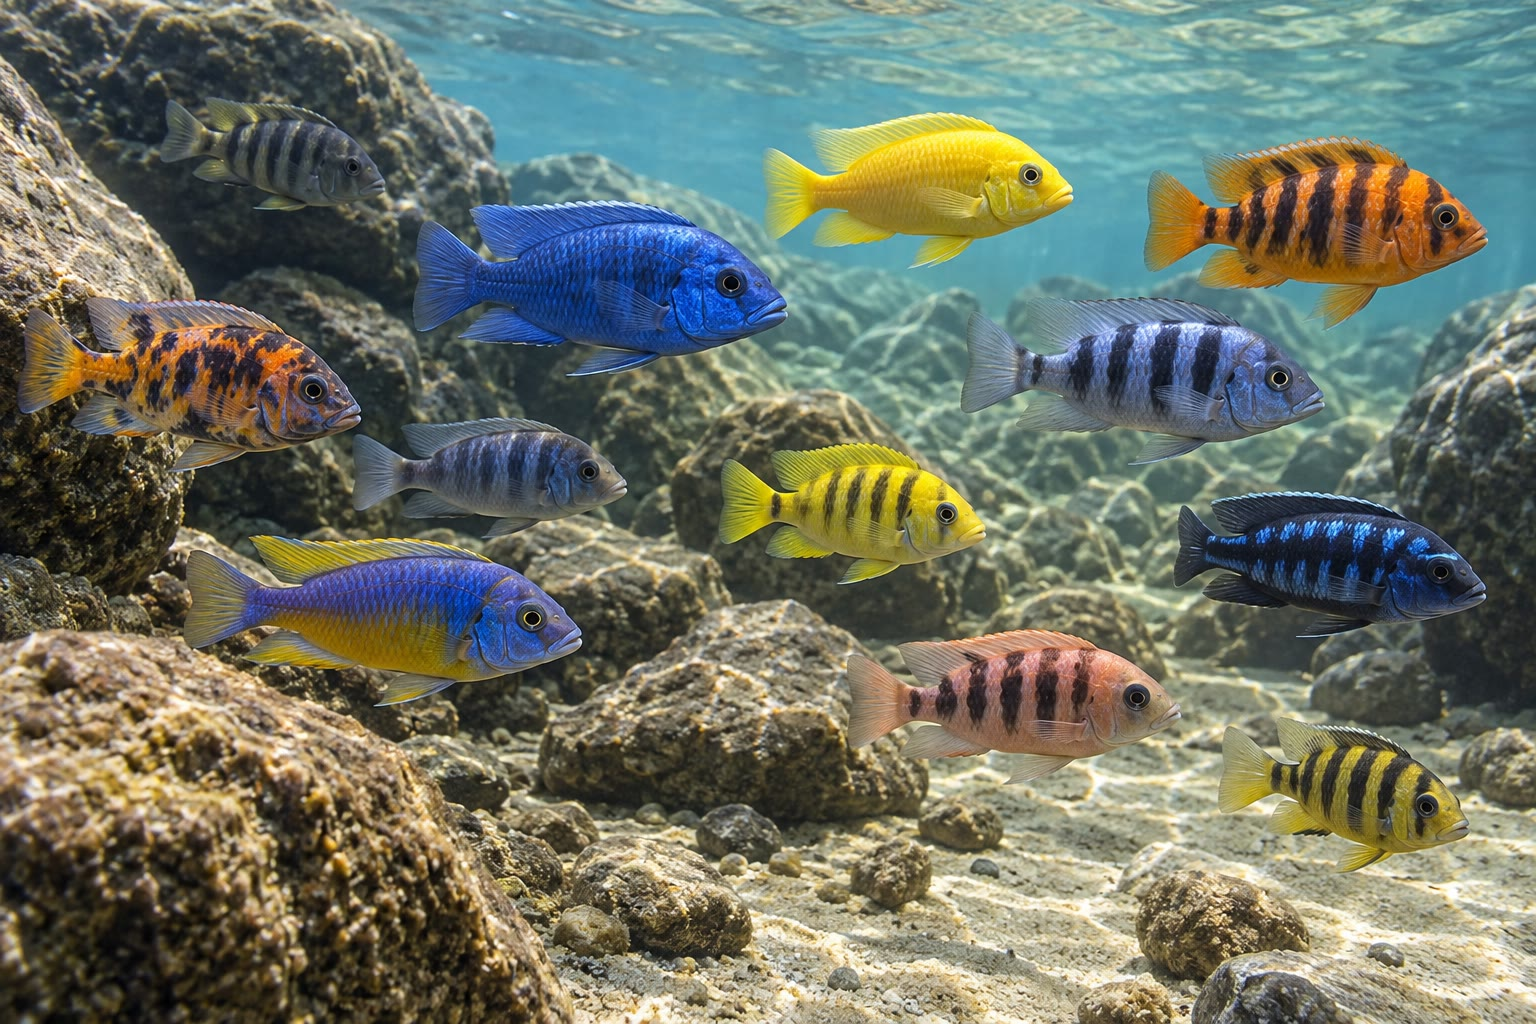
\includegraphics[width=0.6\linewidth]{images/book5/ai/b5-25-cichlids.jpg}

{\small Ciclídeos de um lago africano: centenas de espécies em poucos
milhares de anos, com suas diferenças tiradas em boa parte da variação
que seus ancestrais comuns já carregavam.}
\end{omfigure}

\begin{remark}[O acaso como linha de base]\label{rem:b3:molecular-evolution:remark}
A \omterm{thm:b3:molecular-evolution:neutral}{teoria neutra} não é a afirmação de que a seleção é pouco importante; é
uma afirmação do que acontece quando a seleção está ausente, precisa o
bastante para ser testada. Como a taxa neutra é a taxa de mutação, a
divergência mede tempo; como a mudança neutra preenche os sítios que a
seleção deixa livres, $\omega$ mede restrição; como as linhagens neutras
coalescem a uma taxa conhecida, a discordância das \omterm{prop:b3:molecular-evolution:ils}{árvores gênicas} mede o
tamanho de populações que ninguém viu. A seleção é, então, o que resta
depois de subtraído o acaso --- um gene com $\omega$ acima de um, uma
varredura que esvaziou a variação de uma região, uma árvore que discorda
numa direção que a deriva não explica. O anticongelante do peixe-gelo
antártico, a lisozima estomacal do ruminante e a terceira opsina do
primata são as exceções encontradas assim, e cada uma é a história de um
gene copiado e de um trabalho novo. O resto do genoma é um relógio.
\end{remark}

\section{Exercícios}

\begin{exercise}[$\star$]\label{exo:b3:molecular-evolution:1}
Enuncie a taxa neutra de substituição e explique em palavras por que ela
não depende do tamanho da população.
\end{exercise}

\begin{exercise}[$\star$]\label{exo:b3:molecular-evolution:2}
Defina \omterm{def:b3:genomics:comparative}{ortólogo}, \omterm{def:b3:genomics:comparative}{parálogo} e \omterm{def:b3:molecular-evolution:duplication}{pseudogene}, com um exemplo de cada um na
família das globinas.
\end{exercise}

\begin{exercise}[$\star$]\label{exo:b3:molecular-evolution:3}
O que $\omega = d_{N}/d_{S}$ mede? Interprete $\omega = 0.02$, $\omega = 1.0$ e $\omega = 2.5$, e nomeie um gene de cada tipo.
\end{exercise}

\begin{exercise}[$\star$]\label{exo:b3:molecular-evolution:4}
Por que Kimura concluiu que a maioria das substituições é neutra?
Reenuncie o argumento com os números da abertura do capítulo.
\end{exercise}

\begin{exercise}[$\star\star$]\label{exo:b3:molecular-evolution:5}
$N = 5000$. Calcule a \omterm{thm:b3:molecular-evolution:neutral}{probabilidade de fixação} de uma mutação nova com $s
= 0$, $s = 0.001$, $s = 0.01$ e $s = -0.001$, usando a fórmula de Kimura,
e comente quais são efetivamente neutras.
\end{exercise}

\begin{exercise}[$\star\star$]\label{exo:b3:molecular-evolution:6}
Duas espécies diferem em \qty{12}{\%} dos sítios de um gene cuja taxa
neutra é de \qty{2e-9}{} por sítio por ano. Estime o tempo de divergência
com e sem a correção de Jukes--Cantor. Em que diferença bruta a correção
chega a um fator de dois?
\end{exercise}

\begin{exercise}[$\star\star$]\label{exo:b3:molecular-evolution:7}
Um gene de 300 códons tem 700 sítios não sinônimos e 200 sinônimos. Entre
duas espécies ele mostra 7 diferenças não sinônimas e 10 sinônimas.
Calcule $p_{N}$, $p_{S}$ e $\omega$ (sem correção). Que regime de
seleção? E se as contagens fossem 35 e 10?
\end{exercise}

\begin{exercise}[$\star\star$]\label{exo:b3:molecular-evolution:8}
As sequências neutras de humano e chimpanzé diferem em \qty{1.2}{\%}; a
separação foi há \qty{6.5}{Myr}, com tempo de geração de \qty{25}{yr}.
Estime a taxa de mutação por sítio por geração e o número de mutações
novas num genoma diploide de $6\times 10^{9}$ bases a cada geração.
\end{exercise}

\begin{exercise}[$\star\star$]\label{exo:b3:molecular-evolution:9}
Com $N = \num{50000}$ e $T = \num{100000}$ gerações entre as duas
separações, calcule a fração de \omterm{prop:b3:molecular-evolution:ils}{árvores gênicas} discordantes da \omterm{prop:b3:molecular-evolution:ils}{árvore de
espécies} para humano, chimpanzé e gorila. Que $T$ a tornaria de
\qty{10}{\%}?
\end{exercise}

\begin{exercise}[$\star\star\star$]\label{exo:b3:molecular-evolution:10}
Mostre que a fórmula de Kimura se reduz a $1/2N$ quando $s \to 0$ e a
$2s$ para $4Ns \gg 1$, e que para $s < 0$ com $4N|s| \gg 1$ ela se
comporta como $2|s|\,\mathrm{e}^{-4N|s|}$. Daí estime quão fortemente
deletéria uma mutação precisa ser, numa população de $10^{4}$, para ter
sua \omterm{thm:b3:molecular-evolution:neutral}{probabilidade de fixação} reduzida cem vezes abaixo da neutra.
\end{exercise}

\begin{exercise}[$\star\star\star$]\label{exo:b3:molecular-evolution:11}
Um teste de taxa relativa: um grupo externo $O$ está a uma distância
corrigida de $0.30$ do camundongo e de $0.24$ do humano, e camundongo e
humano estão a $0.20$ um do outro. Calcule os comprimentos dos ramos do
camundongo e do humano desde sua separação (suponha que o ponto de
separação é equidistante de $O$ pelos dois caminhos) e sua razão. Com uma
geração de camundongo de \qty{0.5}{yr} e uma humana de \qty{25}{yr}, o
que um relógio estrito por geração preveria para a razão, e o que a
observação diz sobre as taxas de mutação por geração?
\end{exercise}

\begin{exercise}[$\star\star\star$]\label{exo:b3:molecular-evolution:12}
Um gene duplicado é liberado da restrição ($\omega = 1$) a uma taxa
neutra $k = \qty{2e-9}{}$ por sítio por ano. Numa sequência codificadora
de 1000 bases, quantos anos, aproximadamente, até se esperar o primeiro
códon de parada ou mudança de fase (suponha que cerca de \qty{4}{\%} das
mutações pontuais aleatórias numa sequência codificadora criam um códon
de parada, e ignore as inserções e deleções)? Compare com o tempo que a
seleção tem para encontrar uma função nova e explique por que a maioria
das duplicatas morre.
\end{exercise}

\section{Problema: A Taxa da Mudança}

\begin{problem}[{Problema de fim de semana --- a história de um genoma em
números: a taxa de mutação a partir da divergência humano--chimpanzé, a
carga de substituição de Kimura, as chances de fixação de mutações
selecionadas, o $\omega$ de um gene a partir de contagens de códons, o
relógio lido para uma duplicação e a discordância das árvores gênicas
entre os grandes primatas, terminando na taxa de mutação, no $\omega$ do
gene e na fração discordante}]
\label{pb:b3:molecular-evolution:1}
Dados: divergência neutra humano--chimpanzé $d = 0.012$; separação há
\qty{6.5}{Myr}; geração de \qty{25}{yr}; genoma diploide de $6\times
10^{9}$ bases, \qty{1.5}{\%} codificador. População ancestral $N =
\num{50000}$. Gene: 400 códons, 920 sítios não sinônimos e 280 sinônimos;
diferenças humano--camundongo de 46 não sinônimas e 84 sinônimas.
Separação humano--camundongo há \qty{90}{Myr}. Globina: $\alpha$ e
$\beta$ diferem em \qty{55}{\%} dos sítios de aminoácidos (bruto); taxa
da hemoglobina de \num{1e-9} por sítio por ano. Primatas: $T$ entre as
separações do gorila e do chimpanzé, \num{80000} gerações. Limite de
Haldane: uma substituição selecionada a cada 300 gerações.

\medskip
\noindent\textbf{Parte I --- A taxa.}
\begin{enumerate}
  \item A partir de $d = 2kT$, calcule $k$ por sítio por ano e depois
        $\mu$ por sítio por geração.
  \item Mutações novas por genoma diploide por geração, e quantas delas
        caem em sequência codificadora.
  \item Substituições fixadas por geração em todo o genoma na taxa neutra
        (a população fixa $\mu$ por sítio por geração). Compare com o
        limite de Haldane e tire a conclusão de Kimura.
  \item Numa população de $N = \num{50000}$, quantas mutações neutras
        novas surgem por sítio por geração em toda a população, e que
        fração delas jamais se fixará?
  \item Quanto tempo leva uma mutação neutra destinada a se fixar, em
        gerações e em anos? Compare com o tempo decorrido desde a
        separação humano--chimpanzé.
  \item Explique por que, apesar da questão~5, a divergência entre duas
        espécies mede o tempo desde sua separação, e não o tempo desde a
        fixação de seus alelos.
\end{enumerate}

\medskip
\noindent\textbf{Parte II --- As chances da seleção.}
\begin{enumerate}[resume]
  \item \omterm{thm:b3:molecular-evolution:neutral}{Probabilidade de fixação} de uma mutação neutra em $N = \num{50000}$, e de uma com $s = 0.001$, $s = 0.01$, $s = 0.1$.
  \item Para que $s$ vale $4Ns = 1$? Interprete a fronteira.
  \item Uma mutação deletéria com $s = -0.001$: \omterm{thm:b3:molecular-evolution:neutral}{probabilidade de fixação}
        em relação à neutra. E com $s = -10^{-5}$?
  \item Se uma fração $10^{-5}$ das mutações novas num gene é benéfica
        com $s = 0.01$ e o restante é neutro, que fração das substituições
        nesse gene é adaptativa? Comente quão raramente a seleção aparece
        na sequência, mesmo quando age.
  \item Calcule $p_{N}$ e $p_{S}$ para o gene humano--camundongo, corrija
        cada um com Jukes--Cantor e dê $\omega$.
  \item Interprete $\omega$; e estime a taxa neutra que o $d_{S}$ do gene
        implica (por sítio por ano) usando o tempo de separação. Ela é
        consistente com a questão~1?
\end{enumerate}

\medskip
\noindent\textbf{Parte III --- Relógios e cópias.}
\begin{enumerate}[resume]
  \item Corrija a diferença entre as globinas $\alpha$ e $\beta$ para
        múltiplos acertos (use $d = -\ln(1 - p)$, a versão proteica com
        muitos estados) e date a duplicação com a taxa da hemoglobina.
  \item A data cai perto da origem dos vertebrados mandibulados
        (\qtyrange{450}{500}{Myr}). O que ter cadeias $\alpha$ e $\beta$
        separadas permite que uma cadeia única não permite?
  \item Os fibrinopeptídeos mudam a $8\times 10^{-9}$ por sítio por ano.
        Duas espécies se separaram há \qty{40}{Myr}: diferença bruta
        esperada? Por que essa proteína é inútil para datar separações de
        \qty{500}{Myr}?
  \item A \omterm{def:b3:chromatin-epigenetics:nucleosome}{histona} H4 muda a $10^{-11}$: quantas substituições em 100
        sítios ao longo de \qty{1000}{Myr}? Por que ela é inútil para
        datar separações recentes?
  \item Um gene duplicado deriva com $\omega = 1$ desde o momento da
        duplicação. Se \qty{4}{\%} das substituições em sequência
        codificadora criam paradas, e o gene tem 1200 sítios a uma taxa
        de $2\times
        10^{-9}$ por sítio por ano, estime o tempo esperado
        até o primeiro códon de parada.
  \item Por que a \omterm{def:b3:genomics:comparative}{duplicação do genoma inteiro} dá às duplicatas uma
        chance melhor de sobrevivência que uma única duplicação em
        tandem?
\end{enumerate}

\medskip
\noindent\textbf{Parte IV --- Árvores dentro de árvores.}
\begin{enumerate}[resume]
  \item Probabilidade de que uma linhagem humana e uma de chimpanzé não
        coalesçam nas \num{80000} gerações anteriores à separação do
        gorila.
  \item Fração de \omterm{prop:b3:molecular-evolution:ils}{árvores gênicas} discordantes da \omterm{prop:b3:molecular-evolution:ils}{árvore de espécies}.
        Observado: cerca de \qty{30}{\%}. É consistente?
  \item Das árvores discordantes, que fração agrupa o humano com o gorila
        e que fração agrupa o chimpanzé com o gorila? O que um desvio
        forte da igualdade indicaria?
  \item Se a população ancestral tivesse sido $N = \num{10000}$, que
        fração discordante você esperaria? O que a fração observada diz,
        portanto, sobre os números de nossos ancestrais?
  \item Por que concatenar mil genes num único \omterm{def:b3:bioinformatics:alignment}{alinhamento} dá uma árvore
        confiante, mas possivelmente errada, e o que um método do
        coalescente faz em vez disso?
  \item O DNA neandertal nos humanos não africanos é de cerca de
        \qty{2}{\%}, e as árvores que o carregam agrupam alguns europeus
        com os neandertais mais vezes que os africanos. Por que isso não é
        \omterm{prop:b3:molecular-evolution:ils}{separação incompleta de linhagens}?
  \item Resuma: $\mu$ (questão~1), o $\omega$ do gene (questão~11) e a
        fração discordante (questão~20).
\end{enumerate}
\end{problem}
